\documentclass[14pt]{extreport}
\usepackage{gost}
\usepackage{hyperref}
\usepackage{makecell}
\usepackage{ragged2e}
\usepackage{graphicx}%Вставка картинок правильная
\usepackage{float}%"Плавающие" картинки
\usepackage{wrapfig}%Обтекание фигур (таблиц, картинок и прочего)
\justifying
\makeatletter
\@addtoreset{figure}{part}% Reset figure numbering at every part
\makeatother
\renewcommand{\thefigure}{\arabic{figure}}% Figure number is part.figure
\renewcommand{\thetable}{\arabic{table}}



%Тут можно вставить дополнительные пакеты

\begin{document}
\pagestyle{empty} %  выключаем нумерацию
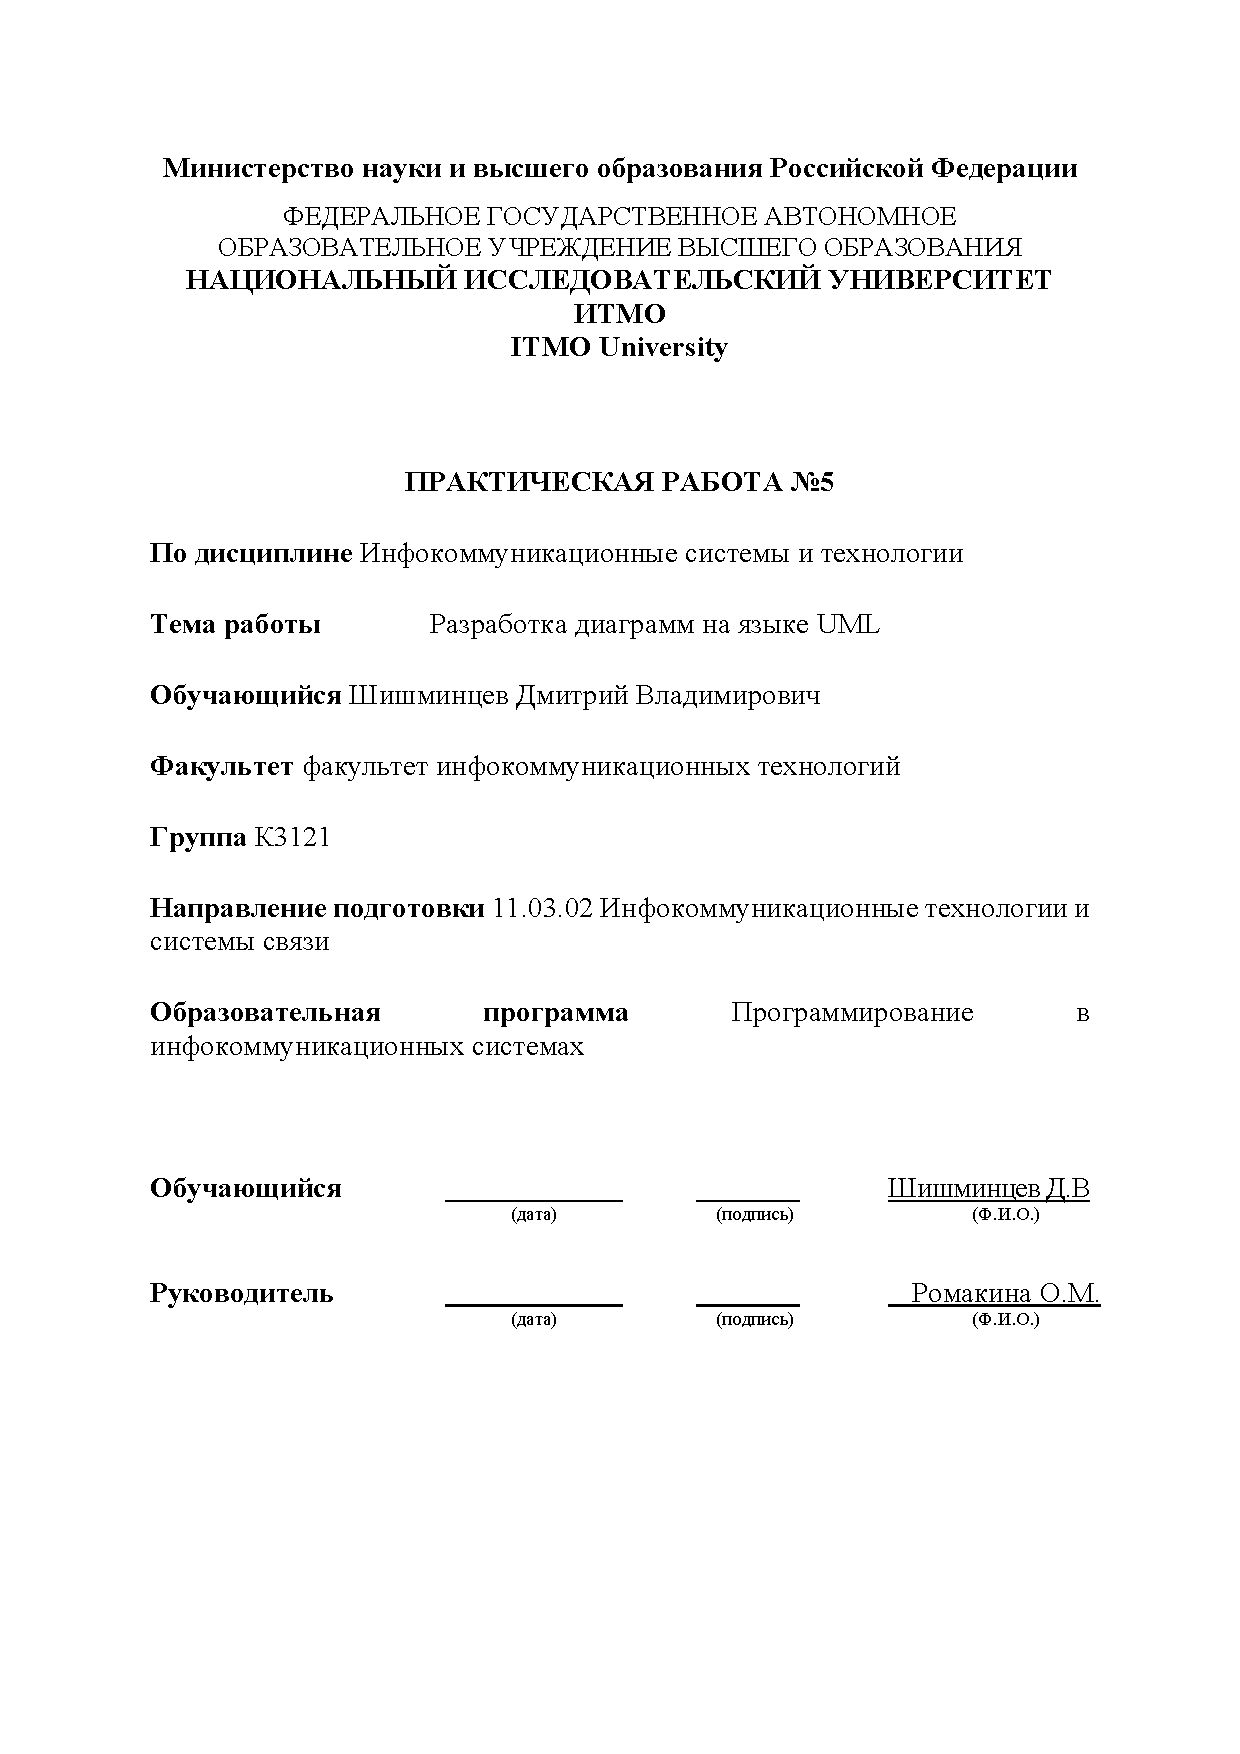
\includepdf[pages=-,pagecommand={}]{title_page.pdf}


\pagestyle{plain} % включаем нумерацию
\tableofcontents
\intro\label{intro} 

Данная практическая работа содержит в себе краткое описание предметной области функционирования и основных пользователей будующей информационной системы, так же была разработана диаграмма прецедентов будующей информационной системы на языке UML и диаграммы активности для ключевых прецедентов.


\chapter{ОПИСАНИЕ ИДЕИ ИНФОРМАЦИОННОЙ СИСТЕМЫ \label{chapter1}}

\section{Основной функционал}

Информационная система MEET ME представляет из себя веб-приложение для планирования встреч с друзьями и родственниками в виде календаря. 
Приложение показывает пересечение свободного времени пользователя с одним или несколькими его друзьями.
C помощью данного приложения пользователь может эффективно планировать встречи со своими друзьями, родственниками или знакомыми не тратя огромное количество времени на согласования времени. 

После создания аккаунта, пользователю будет предложено настроить свое расписание. Пользователь выбирает дни и время, когда он имеет возможность для встречи. 
Настроив свое расписание, пользователь должен добавить своих друзей.  Добавление друзей идет посредством отправки запроса другу на его электронную почту указаную при регистрации аккаунта.

Настроив свое расписание и добавив друзей, пользователю начинают отображаться пересечения в расписании с его друзьями в виде календаря. Пользователю не показывается полностью расписание встреч его друзей ради сохранения приватности. Пользователь может отправить приглашение на встречу своему другу если их свободное время пересекается в приложении. Приглашение отобразится у его друга и он сможет принять или отклонить его. Приняв приглашение у обоих пользователей отобразится встреча в их календаре. 

\section{Основные пользователи}

Информационная система будет иметь только прямых конечных пользователей. Система не требует модераторов, менеджеров и прочих пользователей.
Целевая аудитория данной информационной системы достаточно широка. Основными пользователями будут молодые, общительные люди, которые стараются грамотно распределять свое время (ученики старших классов, студенты, работающая молодежь).


\chapter{ДИАГРАММЫ ВАРИАНТОВ ИСПОЛЬЗОВАНИЯ}

\section{Диаграмма прецедентов}
В данном разделе демонстрируется диаграмма прецедентов [\ref{fig:d1}]  для будующей информационной системы. Диаграмма описывает систему на концептуальном уровне и позволяет понять ее возможности и отношение с актерами.
\begin{figure}[h]   
    \centering
    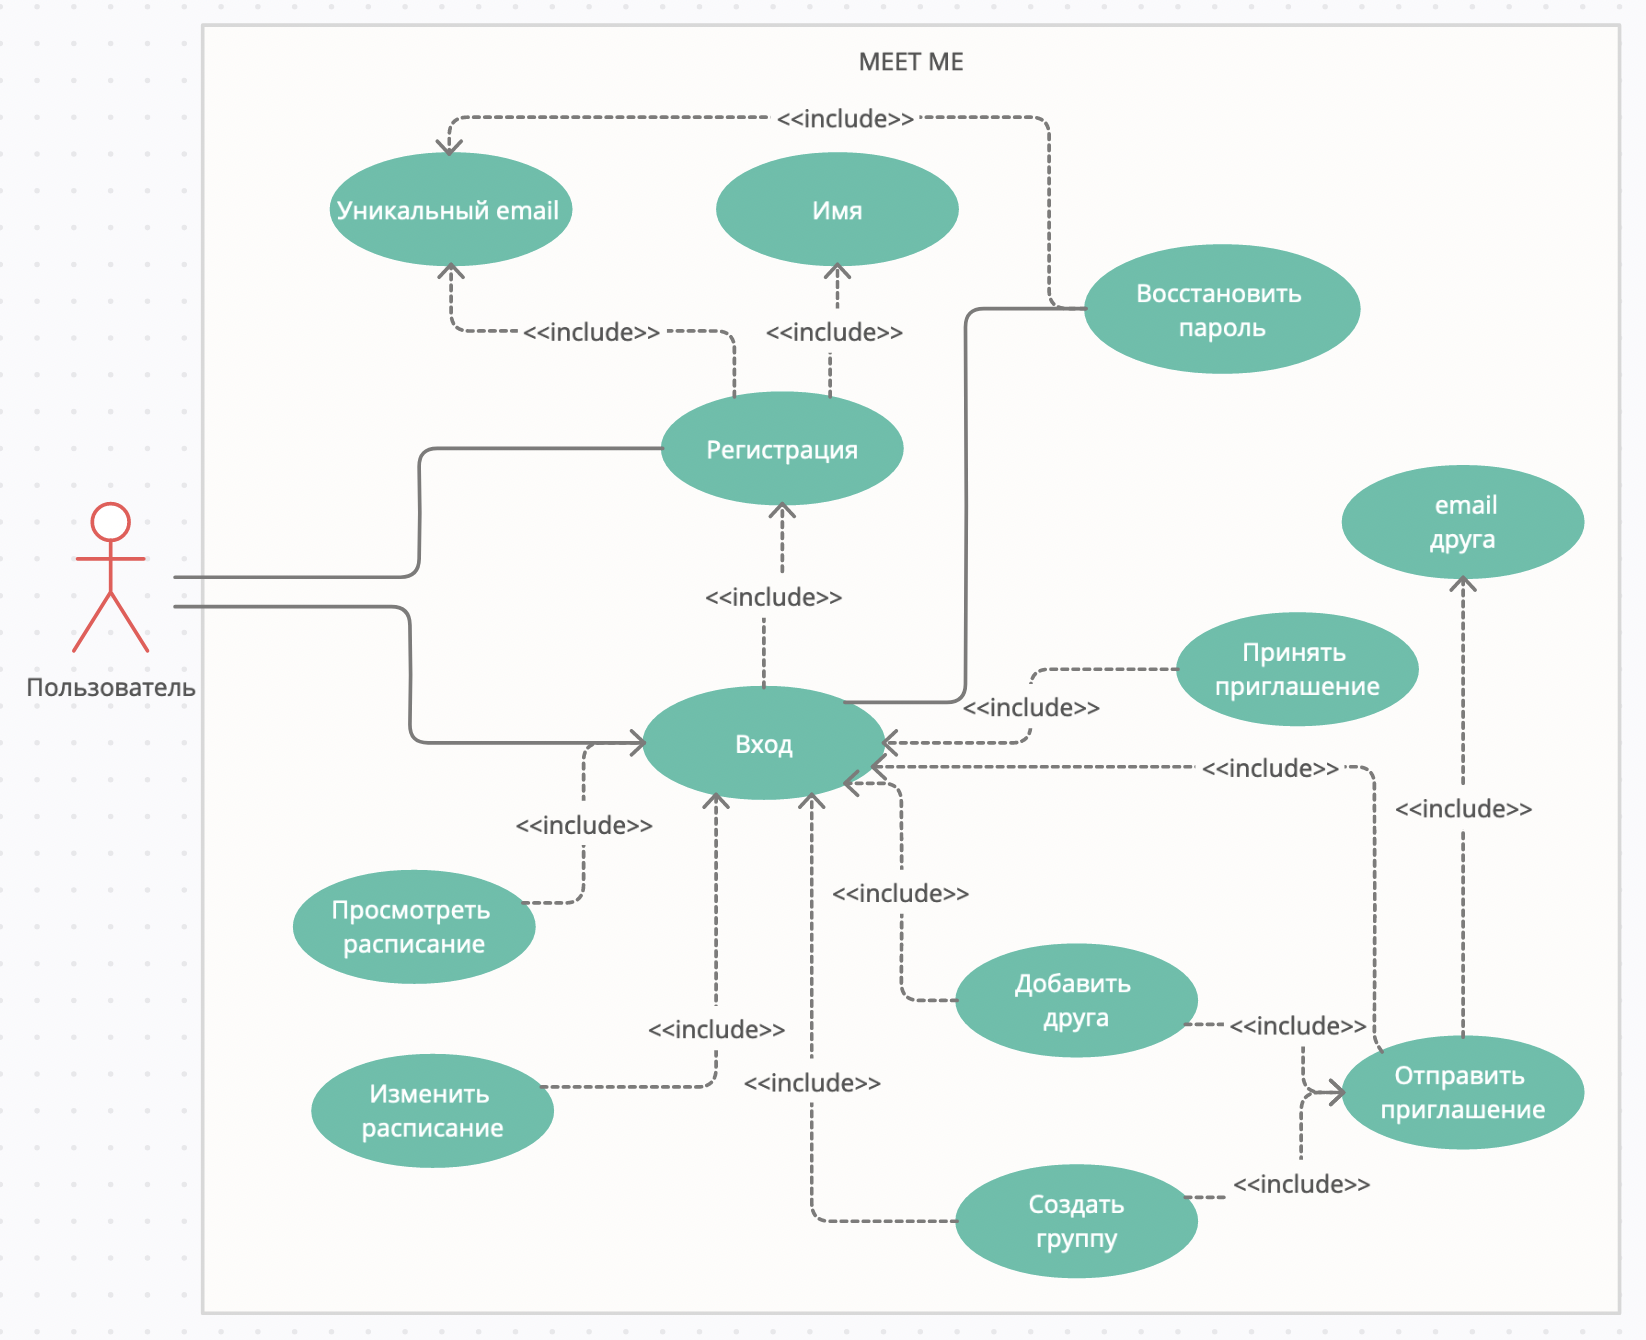
\includegraphics[width=0.8\linewidth]{img/d1.png}
    \caption{ Диаграмма прецедентов}
    \label{fig:d1}
\end{figure}

\section{Диаграммы активности для ключевых прецедентов}
Для ключевых прецедентов были составлены диаграммы активности. Представленные диаграммы отражают динамические аспекты поведения системы.

Диаграмма прецедента <<Вход>> [\ref{fig:d2}] показывает поведение системы при входе пользователя в систему. Если пользователь не зарегистрирован, то система предложит ему создать аккаунт. Если пользователь не может войти в систему, то система предложит ему восстановить пароль.
\begin{figure}[h]   
    \centering
    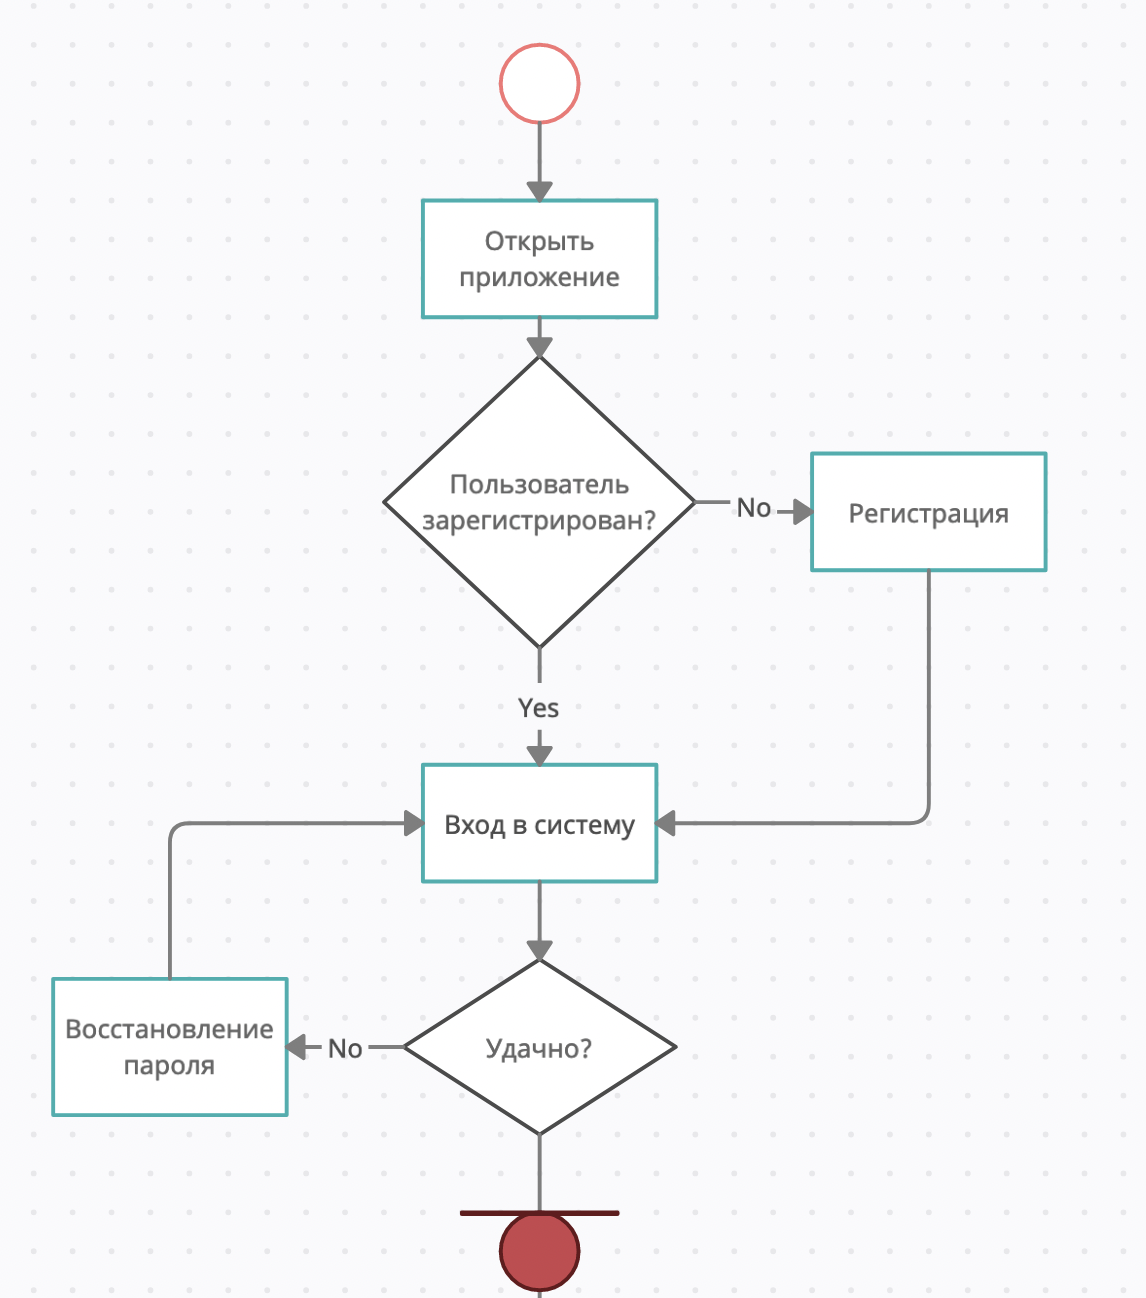
\includegraphics[width=0.94\linewidth]{img/d2.png}
    \caption{ Диаграмма прецедента <<Вход>>}
    \label{fig:d2}
\end{figure}
\newpage 
Диаграмма прецедента <<Просмотреть расписание>> [\ref{fig:d3}] показывает поведение системы при отображении расписания. Если расписание не настроено, то пользователю предложат его настроить. Система отображает запланированные встречи, если они есть, далее если есть пересечения свободного времени с друзьями, то показывает блоки пересечения. 
\begin{figure}[h]   
    \centering
    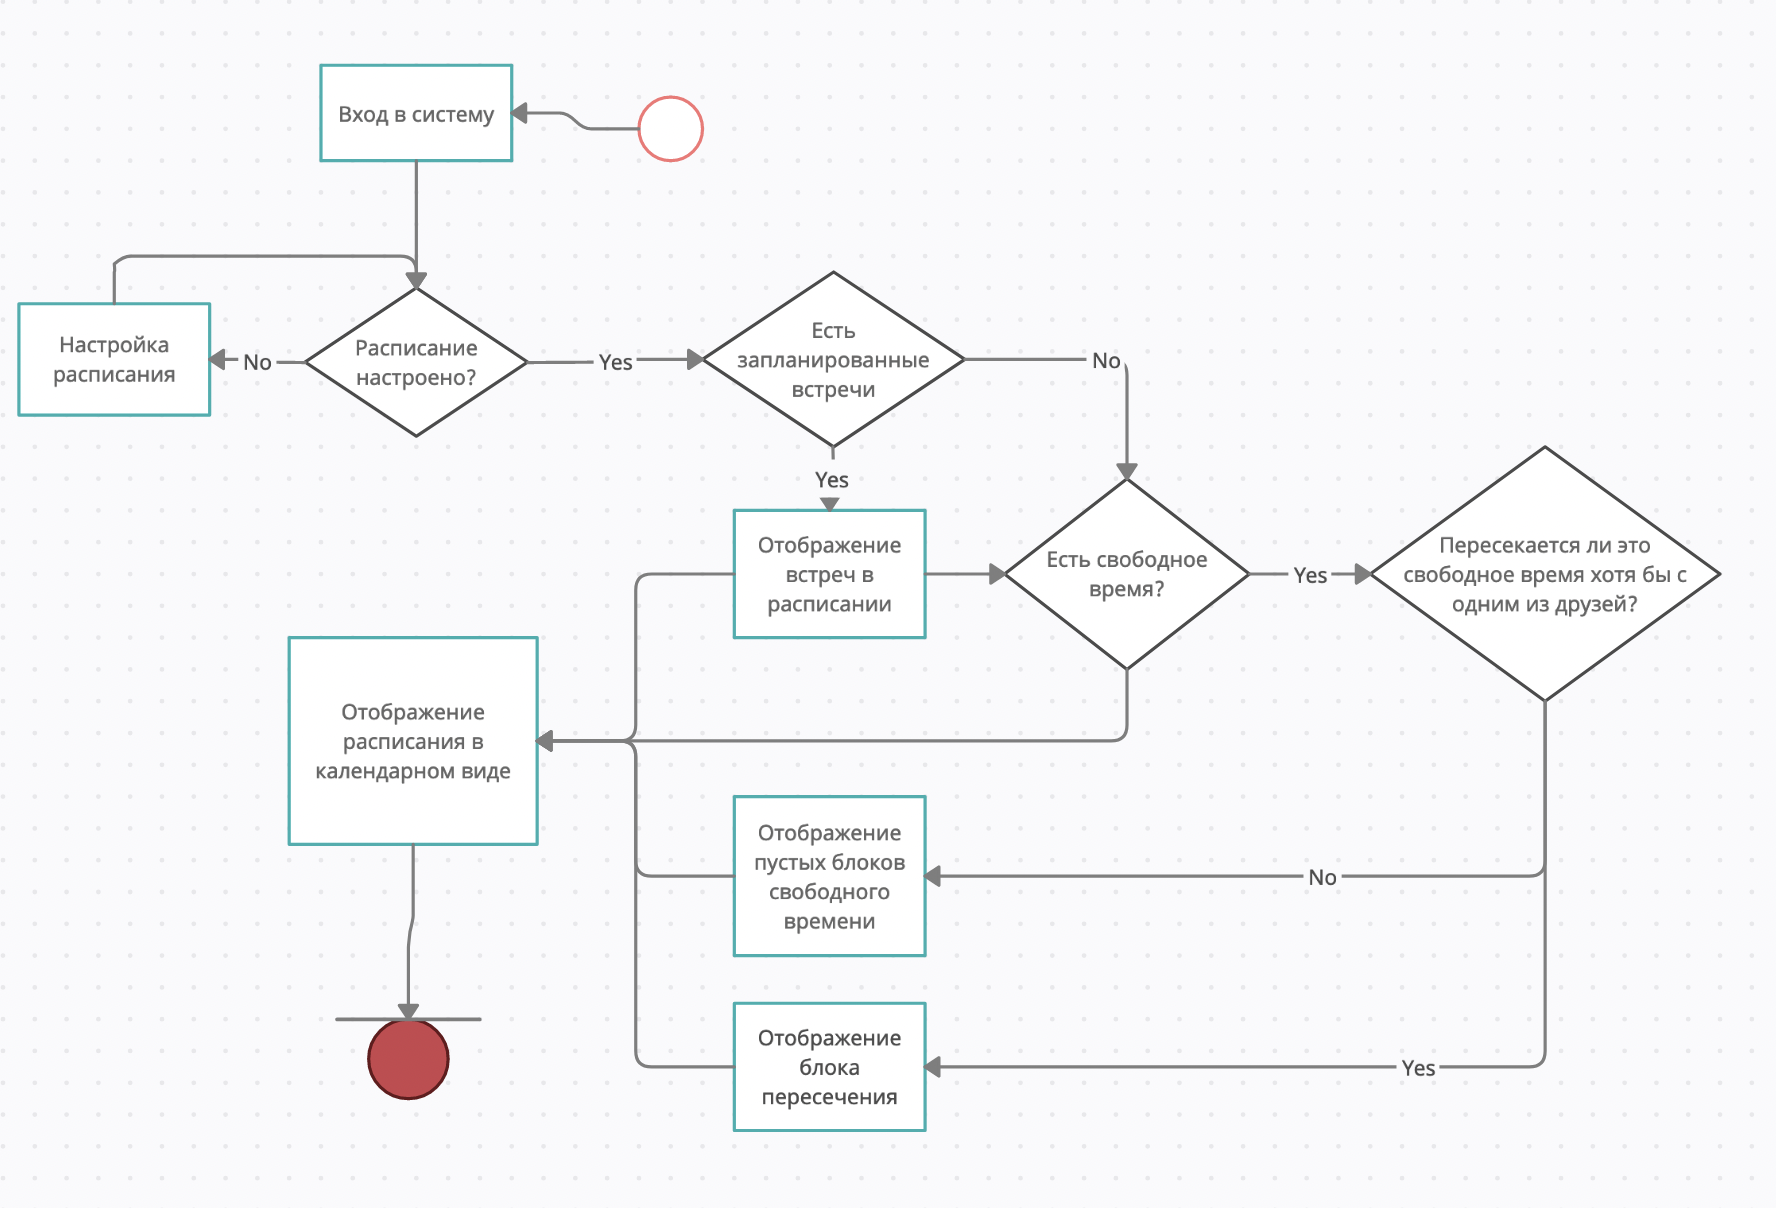
\includegraphics[width=0.94\linewidth]{img/d3.png}
    \caption{ Диаграмма прецедента <<Просмотреть расписание>>}
    \label{fig:d3}
\end{figure}



\conclusions

Был составлен отчет, кратко описана основная предметная область функционирования будующей информационной системы, разработана диаграмма прецедентов на языке UML, а так же диаграммы активности для ключевых прецедентов.

\newpage
\begin{thebibliography}{99}
	\bibitem{bib1} 	UML Use Case Diagram Tutorial | Lucidchart URL: \url{https://www.lucidchart.com/pages/uml-use-case-diagram} (Дата обращения \today)
    \bibitem{bib2} 	UML Activity Diagram Tutorial | Lucidchart URL: \url{https://www.lucidchart.com/pages/uml-activity-diagram} (Дата обращения \today)
\end{thebibliography}

\end{document}
